
%% bare_conf.tex
%% V1.4b
%% 2015/08/26
%% by Michael Shell
%% See:
%% http://www.michaelshell.org/
%% for current contact information.
%%
%% This is a skeleton file demonstrating the use of IEEEtran.cls
%% (requires IEEEtran.cls version 1.8b or later) with an IEEE
%% conference paper.
%%
%% Support sites:
%% http://www.michaelshell.org/tex/ieeetran/
%% http://www.ctan.org/pkg/ieeetran
%% and
%% http://www.ieee.org/

%%*************************************************************************
%% Legal Notice:
%% This code is offered as-is without any warranty either expressed or
%% implied; without even the implied warranty of MERCHANTABILITY or
%% FITNESS FOR A PARTICULAR PURPOSE! 
%% User assumes all risk.
%% In no event shall the IEEE or any contributor to this code be liable for
%% any damages or losses, including, but not limited to, incidental,
%% consequential, or any other damages, resulting from the use or misuse
%% of any information contained here.
%%
%% All comments are the opinions of their respective authors and are not
%% necessarily endorsed by the IEEE.
%%
%% This work is distributed under the LaTeX Project Public License (LPPL)
%% ( http://www.latex-project.org/ ) version 1.3, and may be freely used,
%% distributed and modified. A copy of the LPPL, version 1.3, is included
%% in the base LaTeX documentation of all distributions of LaTeX released
%% 2003/12/01 or later.
%% Retain all contribution notices and credits.
%% ** Modified files should be clearly indicated as such, including  **
%% ** renaming them and changing author support contact information. **
%%*************************************************************************


% *** Authors should verify (and, if needed, correct) their LaTeX system  ***
% *** with the testflow diagnostic prior to trusting their LaTeX platform ***
% *** with production work. The IEEE's font choices and paper sizes can   ***
% *** trigger bugs that do not appear when using other class files.       ***                          ***
% The testflow support page is at:
% http://www.michaelshell.org/tex/testflow/



\documentclass[conference]{IEEEtran}
% Some Computer Society conferences also require the compsoc mode option,
% but others use the standard conference format.
%
% If IEEEtran.cls has not been installed into the LaTeX system files,
% manually specify the path to it like:
% \documentclass[conference]{../sty/IEEEtran}





% Some very useful LaTeX packages include:
% (uncomment the ones you want to load)


% *** MISC UTILITY PACKAGES ***
%
%\usepackage{ifpdf}
% Heiko Oberdiek's ifpdf.sty is very useful if you need conditional
% compilation based on whether the output is pdf or dvi.
% usage:
% \ifpdf
%   % pdf code
% \else
%   % dvi code
% \fi
% The latest version of ifpdf.sty can be obtained from:
% http://www.ctan.org/pkg/ifpdf
% Also, note that IEEEtran.cls V1.7 and later provides a builtin
% \ifCLASSINFOpdf conditional that works the same way.
% When switching from latex to pdflatex and vice-versa, the compiler may
% have to be run twice to clear warning/error messages.






% *** CITATION PACKAGES ***
%
%\usepackage{cite}
% cite.sty was written by Donald Arseneau
% V1.6 and later of IEEEtran pre-defines the format of the cite.sty package
% \cite{} output to follow that of the IEEE. Loading the cite package will
% result in citation numbers being automatically sorted and properly
% "compressed/ranged". e.g., [1], [9], [2], [7], [5], [6] without using
% cite.sty will become [1], [2], [5]--[7], [9] using cite.sty. cite.sty's
% \cite will automatically add leading space, if needed. Use cite.sty's
% noadjust option (cite.sty V3.8 and later) if you want to turn this off
% such as if a citation ever needs to be enclosed in parenthesis.
% cite.sty is already installed on most LaTeX systems. Be sure and use
% version 5.0 (2009-03-20) and later if using hyperref.sty.
% The latest version can be obtained at:
% http://www.ctan.org/pkg/cite
% The documentation is contained in the cite.sty file itself.






% *** GRAPHICS RELATED PACKAGES ***
%
\ifCLASSINFOpdf
  % \usepackage[pdftex]{graphicx}
  % declare the path(s) where your graphic files are
  % \graphicspath{{../pdf/}{../jpeg/}}
  % and their extensions so you won't have to specify these with
  % every instance of \includegraphics
  % \DeclareGraphicsExtensions{.pdf,.jpeg,.png}
\else
  % or other class option (dvipsone, dvipdf, if not using dvips). graphicx
  % will default to the driver specified in the system graphics.cfg if no
  % driver is specified.
  % \usepackage[dvips]{graphicx}
  % declare the path(s) where your graphic files are
  % \graphicspath{{../eps/}}
  % and their extensions so you won't have to specify these with
  % every instance of \includegraphics
  % \DeclareGraphicsExtensions{.eps}
\fi
% graphicx was written by David Carlisle and Sebastian Rahtz. It is
% required if you want graphics, photos, etc. graphicx.sty is already
% installed on most LaTeX systems. The latest version and documentation
% can be obtained at: 
% http://www.ctan.org/pkg/graphicx
% Another good source of documentation is "Using Imported Graphics in
% LaTeX2e" by Keith Reckdahl which can be found at:
% http://www.ctan.org/pkg/epslatex
%
% latex, and pdflatex in dvi mode, support graphics in encapsulated
% postscript (.eps) format. pdflatex in pdf mode supports graphics
% in .pdf, .jpeg, .png and .mps (metapost) formats. Users should ensure
% that all non-photo figures use a vector format (.eps, .pdf, .mps) and
% not a bitmapped formats (.jpeg, .png). The IEEE frowns on bitmapped formats
% which can result in "jaggedy"/blurry rendering of lines and letters as
% well as large increases in file sizes.
%
% You can find documentation about the pdfTeX application at:
% http://www.tug.org/applications/pdftex





% *** MATH PACKAGES ***
%
%\usepackage{amsmath}
% A popular package from the American Mathematical Society that provides
% many useful and powerful commands for dealing with mathematics.
%
% Note that the amsmath package sets \interdisplaylinepenalty to 10000
% thus preventing page breaks from occurring within multiline equations. Use:
%\interdisplaylinepenalty=2500
% after loading amsmath to restore such page breaks as IEEEtran.cls normally
% does. amsmath.sty is already installed on most LaTeX systems. The latest
% version and documentation can be obtained at:
% http://www.ctan.org/pkg/amsmath





% *** SPECIALIZED LIST PACKAGES ***
%
%\usepackage{algorithmic}
% algorithmic.sty was written by Peter Williams and Rogerio Brito.
% This package provides an algorithmic environment fo describing algorithms.
% You can use the algorithmic environment in-text or within a figure
% environment to provide for a floating algorithm. Do NOT use the algorithm
% floating environment provided by algorithm.sty (by the same authors) or
% algorithm2e.sty (by Christophe Fiorio) as the IEEE does not use dedicated
% algorithm float types and packages that provide these will not provide
% correct IEEE style captions. The latest version and documentation of
% algorithmic.sty can be obtained at:
% http://www.ctan.org/pkg/algorithms
% Also of interest may be the (relatively newer and more customizable)
% algorithmicx.sty package by Szasz Janos:
% http://www.ctan.org/pkg/algorithmicx




% *** ALIGNMENT PACKAGES ***
%
%\usepackage{array}
% Frank Mittelbach's and David Carlisle's array.sty patches and improves
% the standard LaTeX2e array and tabular environments to provide better
% appearance and additional user controls. As the default LaTeX2e table
% generation code is lacking to the point of almost being broken with
% respect to the quality of the end results, all users are strongly
% advised to use an enhanced (at the very least that provided by array.sty)
% set of table tools. array.sty is already installed on most systems. The
% latest version and documentation can be obtained at:
% http://www.ctan.org/pkg/array


% IEEEtran contains the IEEEeqnarray family of commands that can be used to
% generate multiline equations as well as matrices, tables, etc., of high
% quality.




% *** SUBFIGURE PACKAGES ***
%\ifCLASSOPTIONcompsoc
%  \usepackage[caption=false,font=normalsize,labelfont=sf,textfont=sf]{subfig}
%\else
%  \usepackage[caption=false,font=footnotesize]{subfig}
%\fi
% subfig.sty, written by Steven Douglas Cochran, is the modern replacement
% for subfigure.sty, the latter of which is no longer maintained and is
% incompatible with some LaTeX packages including fixltx2e. However,
% subfig.sty requires and automatically loads Axel Sommerfeldt's caption.sty
% which will override IEEEtran.cls' handling of captions and this will result
% in non-IEEE style figure/table captions. To prevent this problem, be sure
% and invoke subfig.sty's "caption=false" package option (available since
% subfig.sty version 1.3, 2005/06/28) as this is will preserve IEEEtran.cls
% handling of captions.
% Note that the Computer Society format requires a larger sans serif font
% than the serif footnote size font used in traditional IEEE formatting
% and thus the need to invoke different subfig.sty package options depending
% on whether compsoc mode has been enabled.
%
% The latest version and documentation of subfig.sty can be obtained at:
% http://www.ctan.org/pkg/subfig




% *** FLOAT PACKAGES ***
%
%\usepackage{fixltx2e}
% fixltx2e, the successor to the earlier fix2col.sty, was written by
% Frank Mittelbach and David Carlisle. This package corrects a few problems
% in the LaTeX2e kernel, the most notable of which is that in current
% LaTeX2e releases, the ordering of single and double column floats is not
% guaranteed to be preserved. Thus, an unpatched LaTeX2e can allow a
% single column figure to be placed prior to an earlier double column
% figure.
% Be aware that LaTeX2e kernels dated 2015 and later have fixltx2e.sty's
% corrections already built into the system in which case a warning will
% be issued if an attempt is made to load fixltx2e.sty as it is no longer
% needed.
% The latest version and documentation can be found at:
% http://www.ctan.org/pkg/fixltx2e


%\usepackage{stfloats}
% stfloats.sty was written by Sigitas Tolusis. This package gives LaTeX2e
% the ability to do double column floats at the bottom of the page as well
% as the top. (e.g., "\begin{figure*}[!b]" is not normally possible in
% LaTeX2e). It also provides a command:
%\fnbelowfloat
% to enable the placement of footnotes below bottom floats (the standard
% LaTeX2e kernel puts them above bottom floats). This is an invasive package
% which rewrites many portions of the LaTeX2e float routines. It may not work
% with other packages that modify the LaTeX2e float routines. The latest
% version and documentation can be obtained at:
% http://www.ctan.org/pkg/stfloats
% Do not use the stfloats baselinefloat ability as the IEEE does not allow
% \baselineskip to stretch. Authors submitting work to the IEEE should note
% that the IEEE rarely uses double column equations and that authors should try
% to avoid such use. Do not be tempted to use the cuted.sty or midfloat.sty
% packages (also by Sigitas Tolusis) as the IEEE does not format its papers in
% such ways.
% Do not attempt to use stfloats with fixltx2e as they are incompatible.
% Instead, use Morten Hogholm'a dblfloatfix which combines the features
% of both fixltx2e and stfloats:
%
% \usepackage{dblfloatfix}
% The latest version can be found at:
% http://www.ctan.org/pkg/dblfloatfix




% *** PDF, URL AND HYPERLINK PACKAGES ***
%
%\usepackage{url}
% url.sty was written by Donald Arseneau. It provides better support for
% handling and breaking URLs. url.sty is already installed on most LaTeX
% systems. The latest version and documentation can be obtained at:
% http://www.ctan.org/pkg/url
% Basically, \url{my_url_here}.




% *** Do not adjust lengths that control margins, column widths, etc. ***
% *** Do not use packages that alter fonts (such as pslatex).         ***
% There should be no need to do such things with IEEEtran.cls V1.6 and later.
% (Unless specifically asked to do so by the journal or conference you plan
% to submit to, of course. )


% correct bad hyphenation here
\hyphenation{op-tical net-works semi-conduc-tor}
\usepackage{graphicx}
\usepackage{float}
\usepackage{mdframed}
\usepackage{listings}

\usepackage[utf8]{inputenc}
\usepackage[T1]{fontenc}
\usepackage[french]{babel}
\usepackage{graphicx}
\usepackage{geometry}
\usepackage{amsmath}
\usepackage{enumitem}
\usepackage{xcolor}
\usepackage{float}
\usepackage{mdframed}
\usepackage{listings}
\usepackage{xcolor}
\usepackage{ulem}
\usepackage{soul}

\definecolor{codebackground}{rgb}{0.95,0.95,0.95}

\lstdefinestyle{terminal}{
  backgroundcolor=\color{codebackground},
  basicstyle=\ttfamily\small,
  frame=none,
  breaklines=true,
  columns=fullflexible,
  postbreak=\mbox{\textcolor{red}{$\hookrightarrow$}\space},
  showstringspaces=false,
  captionpos=b,
  escapeinside={(*@}{@*)},
  numbers=left,
  numberstyle=\tiny,
  numbersep=5pt
}

\geometry{hmargin=2.5cm,vmargin=1.5cm}

\begin{document}
%
% paper title
% Titles are generally capitalized except for words such as a, an, and, as,
% at, but, by, for, in, nor, of, on, or, the, to and up, which are usually
% not capitalized unless they are the first or last word of the title.
% Linebreaks \\ can be used within to get better formatting as desired.
% Do not put math or special symbols in the title.
\title{Écouter parler une IA ou comment mesurer la diversité expressive des modèles de langage automatiques}

% author names and affiliations
% use a multiple column layout for up to three different
% affiliations
\author{\IEEEauthorblockN{Mathias Aurand-Augier}
\IEEEauthorblockA{School of Computer Engineering\\
TELECOM Nancy\\
Villers-les-Nancy, France\\
mathias.aurand-augier@telecomnancy.eu}
\and
\IEEEauthorblockN{Théo Hornberger}
\IEEEauthorblockA{School of Computer Engineering\\
TELECOM Nancy\\
Villers-les-Nancy, France\\
theo.hornberger@telecomnancy.eu}
\and
\IEEEauthorblockN{Terry Tempestini}
\IEEEauthorblockA{School of Computer Engineering\\
TELECOM Nancy\\
Villers-les-Nancy, France\\
terry.tempestini@telecomnancy.eu}
\and}

% conference papers do not typically use \thanks and this command
% is locked out in conference mode. If really needed, such as for
% the acknowledgment of grants, issue a \IEEEoverridecommandlockouts
% after \documentclass

% for over three affiliations, or if they all won't fit within the width
% of the page, use this alternative format:
% 
%\author{\IEEEauthorblockN{Michael Shell\IEEEauthorrefmark{1},
%Homer Simpson\IEEEauthorrefmark{2},
%James Kirk\IEEEauthorrefmark{3}, 
%Montgomery Scott\IEEEauthorrefmark{3} and
%Eldon Tyrell\IEEEauthorrefmark{4}}
%\IEEEauthorblockA{\IEEEauthorrefmark{1}School of Electrical and Computer Engineering\\
%Georgia Institute of Technology,
%Atlanta, Georgia 30332--0250\\ Email: see http://www.michaelshell.org/contact.html}
%\IEEEauthorblockA{\IEEEauthorrefmark{2}Twentieth Century Fox, Springfield, USA\\
%Email: homer@thesimpsons.com}
%\IEEEauthorblockA{\IEEEauthorrefmark{3}Starfleet Academy, San Francisco, California 96678-2391\\
%Telephone: (800) 555--1212, Fax: (888) 555--1212}
%\IEEEauthorblockA{\IEEEauthorrefmark{4}Tyrell Inc., 123 Replicant Street, Los Angeles, California 90210--4321}}




% use for special paper notices
%\IEEEspecialpapernotice{(Invited Paper)}




% make the title area
\maketitle
%\tableofcontents
\newpage

% As a general rule, do not put math, special symbols or citations
% in the abstract
\begin{abstract}
The abstract goes here.
\end{abstract}

% no keywords




% For peer review papers, you can put extra information on the cover
% page as needed:
% \ifCLASSOPTIONpeerreview
% \begin{center} \bfseries EDICS Category: 3-BBND \end{center}
% \fi
%
% For peerreview papers, this IEEEtran command inserts a page break and
% creates the second title. It will be ignored for other modes.
\IEEEpeerreviewmaketitle



\section{Introduction}
% no \IEEEPARstart
This demo file is intended to serve as a ``starter file''
for IEEE conference papers produced under \LaTeX\ using
IEEEtran.cls version 1.8b and later.
% You must have at least 2 lines in the paragraph with the drop letter
% (should never be an issue)
I wish you the best of success.

\hfill mds
 
\hfill August 26, 2015

\subsection{Subsection Heading Here}
Subsection text here.


\subsubsection{Subsubsection Heading Here}
Subsubsection text here.


\section {Motivation}

Considérons un professeur de français corrigeant une rédaction produite par un élève sur un sujet quelconque, comment évalue-t-il la qualité de cette rédaction ? 
Celui-ci dirait sûrement qu'il se base sur la richesse du vocabulaire, la syntaxe, la cohérence, la pertinence, la clarté, la concision, la précision, la variété des structures de phrases, autant de concept relativement difficile à mesurer quantitativement et souvent basé sur l'interprétation de chacun. \\

Pourtant, la compréhension de ces concepts conditionnent dans une certaine mesure la faculté de l'élève à progresser, comment peut il à l'avenir améliorer sa "cohérence" si la définition du terme n'est pas claire à ses yeux.\\

En ce sens, remplaçons le professeur par un programme informatique et l'élève par un modèle de langage automatique, comment un programme pourrait il évaluer la qualité d'un texte produit par un autre programme ?
Il faudrait pour cela définir des critères quantitatif de "qualité" d'un texte.\\

Une méthode possible d'évaluation pourrait se baser sur des références : il ne s'agirait alors pas d'évaluer la qualité d'un texte en lui même, mais plutôt de se demander si un texte semble "de meilleure qualité" qu'un autre.
Pour illustrer ce principe, nous avons à notre disposition 5 générateurs de texte, chacun ayant une qualité de sortie différente. Chaque générateur produit un commentaire relatif à une image donnée.
Le but est de mettre en évidence certains signes de qualités des textes par rapport aux autres.

\section {La notion de "qualité" d'un texte}

\subsection {Richesse du vocabulaire}

Pour évaluer la "qualité" d'un texte, on peut commencer par évaluer la richesse du vocabulaire. 
Par richesse du vocabulaire, on peut entendre plusieurs choses, en effet plusieurs méthodes peuvent être utilisé pour évaluer la richesse du vocabulaire. 
Dans un premier temps, on peut compter le nombre de mots différents généré par chaque intelligence artificielle. 

On obtient les résultats suivants : 

\vspace{5mm}

\begin{mdframed}
  \begin{lstlisting}[style=terminal]
    Number of words in BART_1:  433
    Number of words in BART_2:  483
    Number of words in T5_1:  295
    Number of words in T5_2:  310
    Number of words in FST:  194

    Number of words in total:  863
  \end{lstlisting}
\end{mdframed}

\vspace{5mm}

Avec les résultats obtenus, on observe que BART\_2 et BART\_1 ont un lexique plus variés, suivi de T5\_2, T5\_1 et FST. Cela pourrait indiquer que BART\_2 et BART\_1 ont un vocabulaire plus riche que les autres, et qu'elles emploient alors des mots plus variés.\\

Néanmoins, cette méthode n'est que très superficielle, car elle ne prend pas en compte la fréquence d'apparition des mots ni la longueur de la phrase.

Aussi tentons d'évaluer des caractéristiques statistiques basiques comme la moyenne, la médiane et l'écart type du nombre de mots par phrase générée par chaque IA. Cela pourrait éventuellement expliquer la richesse du vocabulaire de chaque IA.

En effet, la longueur d'une phrase peut cacher une certaine complexité syntaxique, ainsi qu'un contenu explicatif de l'image commenté plus fourni : le fond serait alors de meilleur qualité. Voyons ce que cela donne : 

\vspace{5mm}

%\begin{mdframed}
%  \begin{lstlisting}[style=terminal]
%    Average length of sentences in BART_1 : 11.752
%    Average length of sentences in BART_2 : 13.295
%    Average length of sentences in T5_1 : 14.149
%    Average length of sentences in T5_2 : 11.261
%    Average length of sentences in FST : 7.402
%  \end{lstlisting}
%\end{mdframed}

\begin{figure}[H]
  \centering
  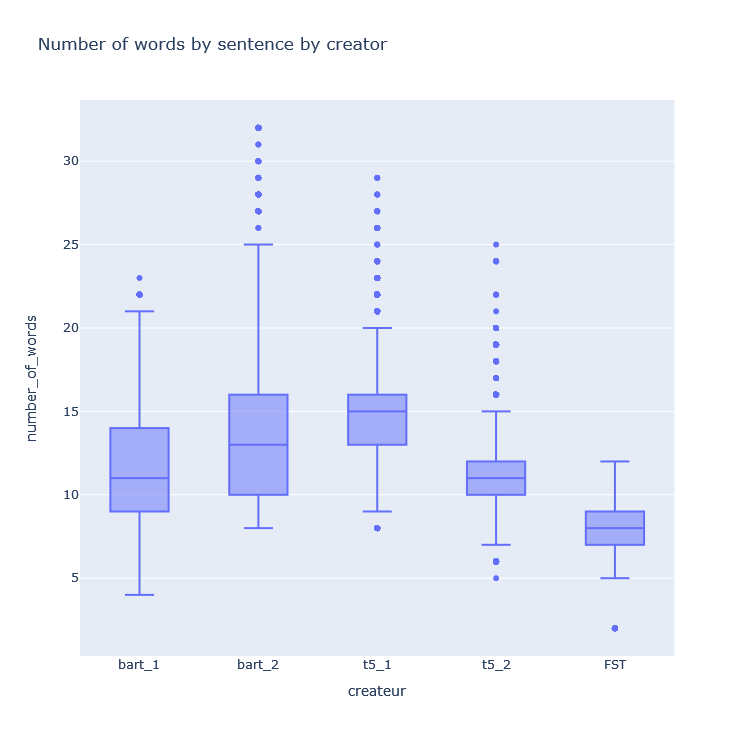
\includegraphics[width=0.5\textwidth]{images/boxplot_sentences.png}
  \caption{Boîte à moustache de la longueur des phrases générées par chaque IA}
  \end{figure}

\vspace{5mm}

Les résultats sont très interessants puisque l'on peut voir que la génération T5\_1 a les phrases les plus longues en moyenne et pourtant un des vocabulaire le plus pauvre, ce qui pourrait être le signe d'une répétition accru des mêmes mots. 
Les différences de longueurs entre BART\_1 et BART\_2 sont également interessantes, puisqu'elle pourrait expliquer le différentiel de vocabulaire entre les deux modèles.
Ensuite, la longueur des phrases de FST est la plus faible, ce qui pourrait expliquer la pauvreté de son vocabulaire.

Il peut être aussi interessant d'étudier la fréquence d'utilisation des mots les plus fréquents. On peut pour cela utiliser un diagramme à barres empilées (on met ainsi en évidence la contribution de chaque IA à l'utilisation globale de chaque mot).

\vspace{5mm}

\begin{figure}[H]
\centering
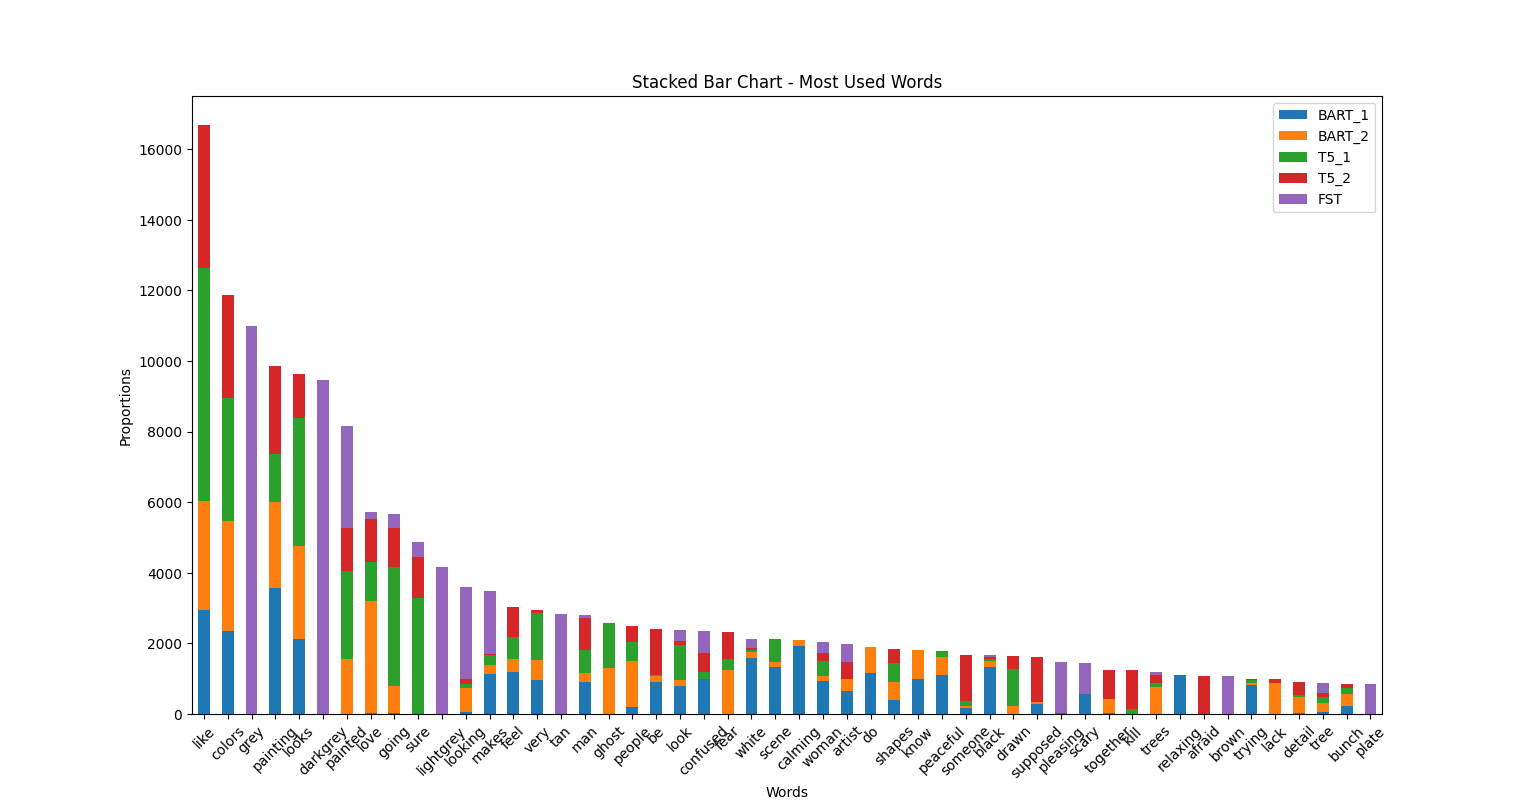
\includegraphics[width=0.5\textwidth]{images/stacked_bars_most_used_words.png}
\caption{Matrice de similarité entre les phrases générées par BART\_1}
\end{figure}

\vspace{5mm}

Un fait particulièrement interessant visible sur ce diagramme est que certains des mots les plus fréquents tel que "grey", "darkgrey", "lightgrey" ne sont utilisé que par FST. Cela révèle une focalisation excessive sur la couleur grise qui n'est apriori une couleur plus présente en générale dans les oeuvres. 
La pertinence des réponses de FST peut donc remise en question sachant qu'elle semble concentrée sur les mêmes caractéristiques, cela peut également expliquer la pauvreté du vocabulaire chez FST.

\subsection {Diversité syntaxique au sein d'une même IA}

Une manière interessante de mesurer la capacité d'une intelligence à générer des réponses différentes est de comparer ses propres réponses entre elles : si les phrases sont globalement proche, cela signifie que l'IA a tendance à répéter les mêmes structures de phrases, et donc à manquer de diversité syntaxique.
Voici un exemple : 

\vspace{5mm}

\begin{figure}[H]
\centering
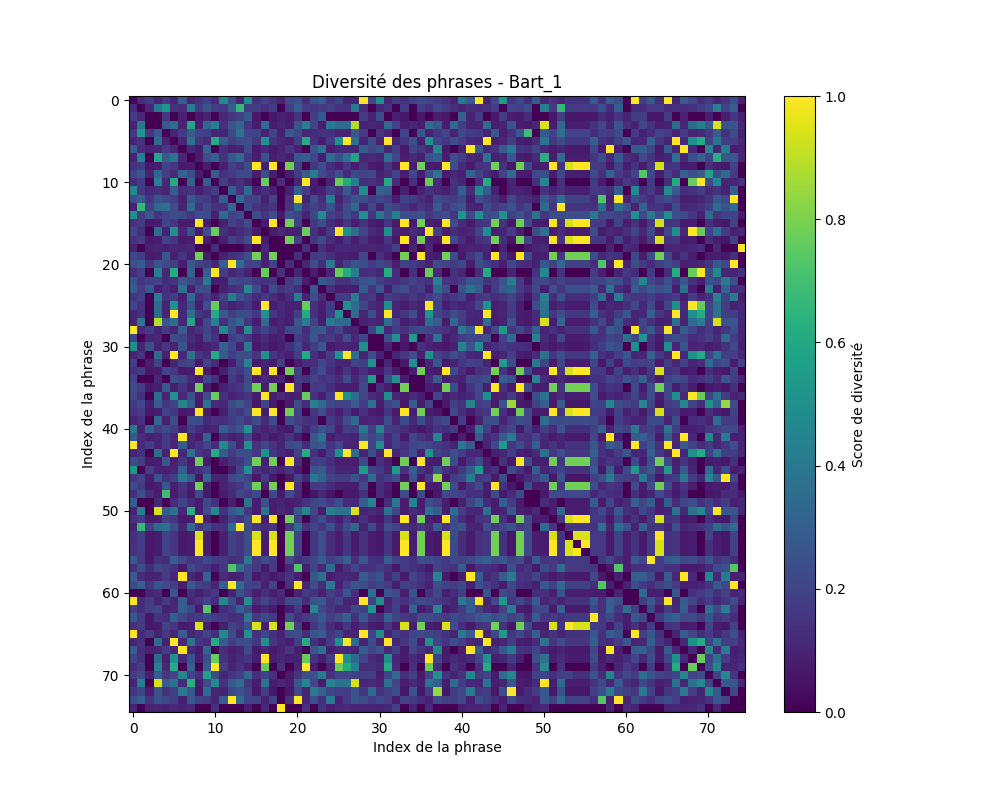
\includegraphics[width=0.6\textwidth]{images/diversity_matrix_bart_1.png}
\caption{Matrice de similarité entre les phrases générées par BART\_1}
\end{figure}

\vspace{5mm}

On remarque ici que la matrice de diversité est relativement sombre, donc proche de 0, ce qui signifie que les phrases générées par BART\_1 sont relativement différentes les unes des autres, démontrant ainsi une certaine capacité à renouveler ses structures phrastiques.

\vspace{5mm}

\begin{figure}[H]
\centering
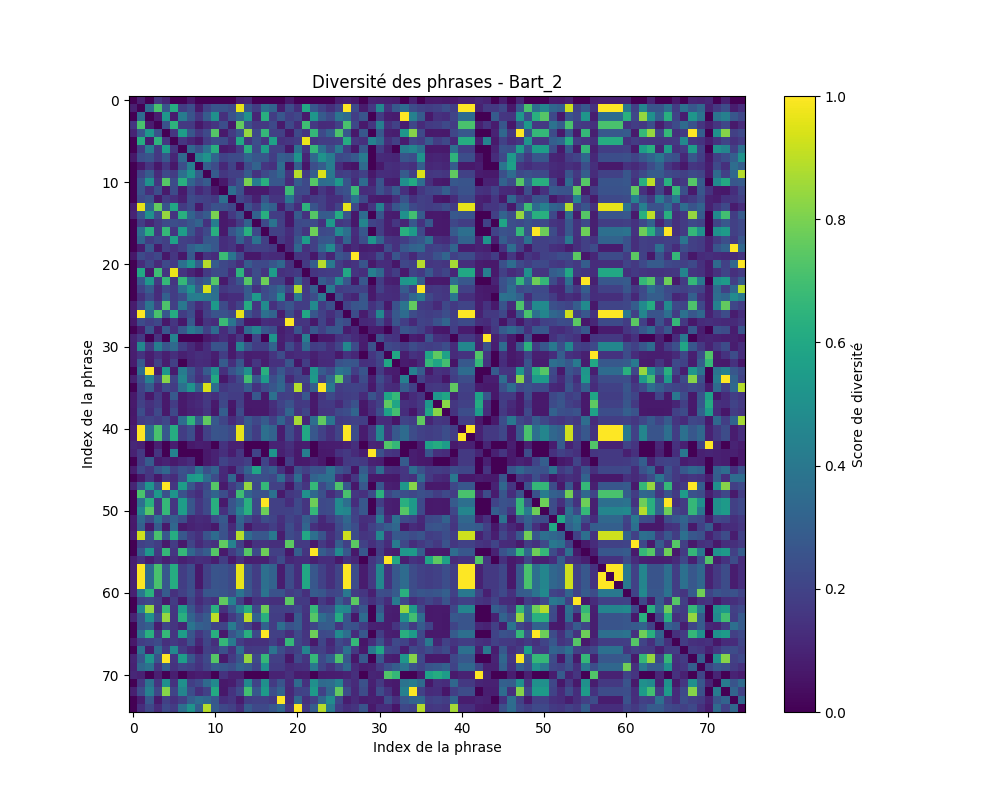
\includegraphics[width=0.6\textwidth]{images/diversity_matrix_bart_2.png}
\caption{Matrice de similarité entre les phrases générées par BART\_2}
\end{figure}

\vspace{5mm}

Ce qui est remarquable pour cette matrice est qu'elle est globalement plus claire que la précédente mais reste néanmoins assez sombre : les phrases sont donc relativement différentes.

\vspace{5mm}

\begin{figure}[H]
\centering
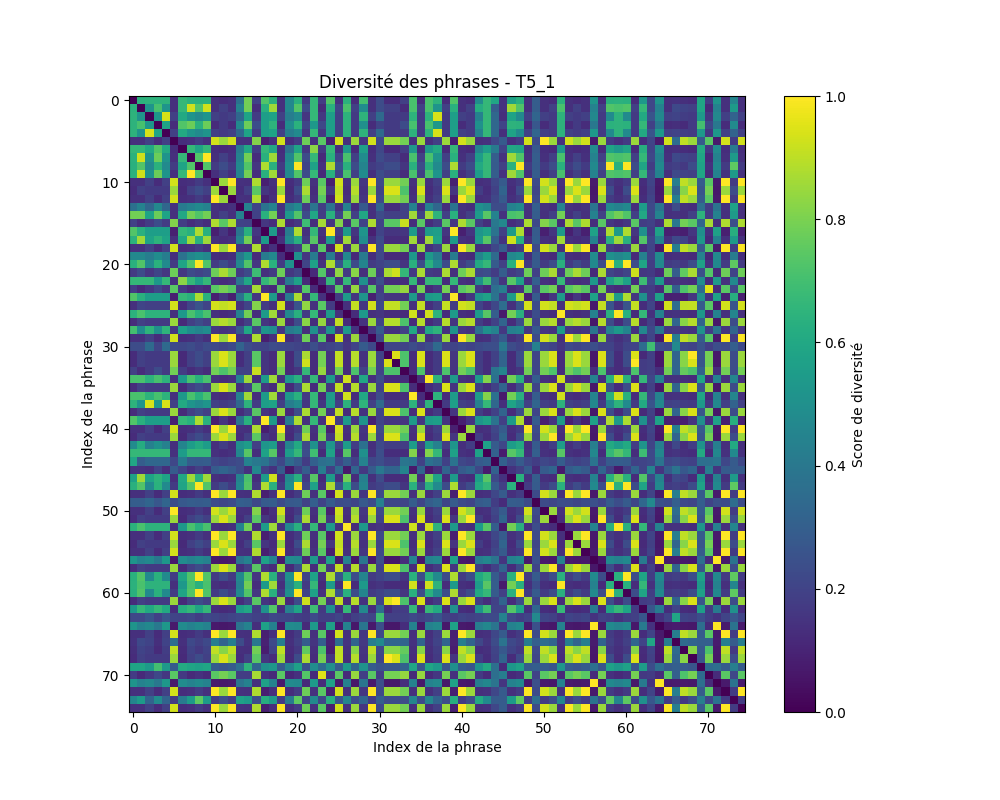
\includegraphics[width=0.6\textwidth]{images/diversity_matrix_t5_1.png}
\caption{Matrice de similarité entre les phrases générées par T5\_1}
\end{figure}

\vspace{5mm}

En revanche, ici il est clair que la matrice a une couleur beaucoup plus claire, ce qui montre que les réponses générées par T5\_1 sont répétitives. Pourtant, quelques points sombres montre qu'elle est capable de se renouveler mais cela semble 
ici ponctuel et non récurrent.

\vspace{5mm}

\begin{figure}[H]
\centering
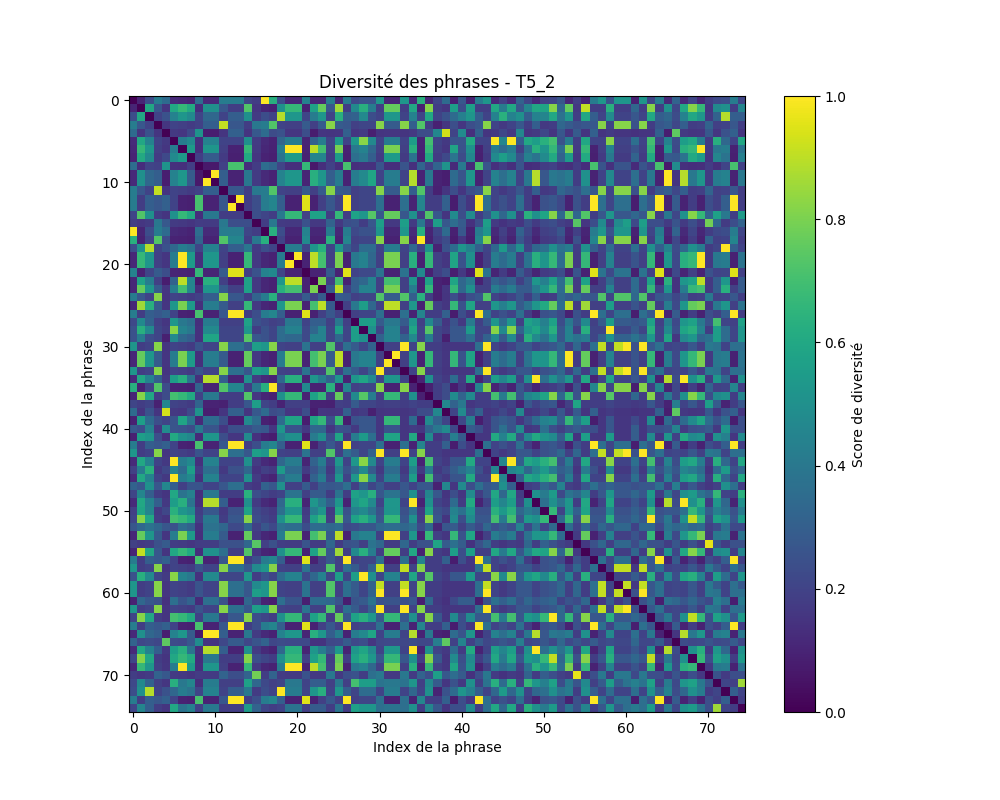
\includegraphics[width=0.5\textwidth]{images/diversity_matrix_t5_2.png}
\caption{Matrice de similarité entre les phrases générées par T5\_2}
\end{figure}

\vspace{5mm}

La matrice de T5\_2 est très similaire à celle de T5\_1, ce qui montre que T5\_2 a également tendance à répéter les mêmes structures de phrases.

\vspace{5mm}

\begin{figure}[H]
\centering
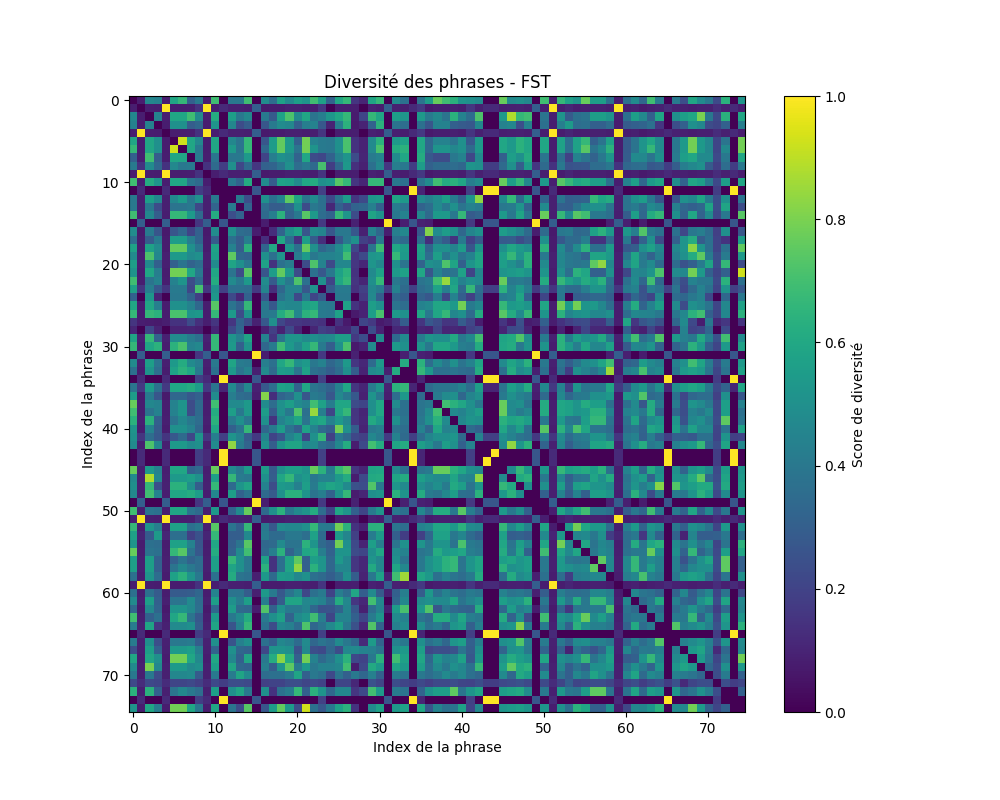
\includegraphics[width=0.6\textwidth]{images/diversity_matrix_FST.png}
\caption{Matrice de similarité entre les phrases générées par FST}
\end{figure}

\vspace{5mm}

De même, la matrice de FST est très similaire à celle de T5\_1 et T5\_2, ce qui montre que FST a également tendance à répéter les mêmes structures de phrases.

\subsection {Mesure de similitude entre les différentes intelligences artificielles}



\subsection {Mesure de similitude au sein des phrases générées par une même IA}
\subsection {}
\subsection {}
\subsection {}

\section {Introduction}





\vspace{5mm}


\section{Analyse de la proximité des phrases générées par les IA}

Dans un premier temps, nous avons effectué une comparaison des réponses des IA concernant une image donnée. L'objectif principal est de déterminer le degré de similarité ou de divergence entre les phrases générées par les différentes IA. Cette comparaison permet non seulement de mesurer la proximité entre les IA deux à deux, mais aussi de déterminer si certaines IA se distinguent des autres.\\

Cependant, il est important de noter que ces mesures ne reflètent pas la "qualité" intrinsèque d'une phrase donnée. Elles ne fournissent qu'une indication de la proximité entre les phrases générées par les différentes IA. Néanmoins, ces mesures sont utiles pour étudier le comportement des IA et identifier d'éventuelles similitudes ou différences marquées entre elles.

\subsection{Utilisation de la métrique ROUGE}

La première métrique utilisée dans notre étude est ROUGE (Recall-Oriented Understudy for Gisting Evaluation). Cette technique compare la similarité entre une phrase de référence et celle générée par l'IA. Elle se base sur le comptage des chevauchements de mots (appelés n-grammes) ou de groupes de mots, selon les paramètres définis. La métrique ROUGE utilise le rappel, la précision et la F-mesure pour évaluer la similarité.\\

Dans notre cas, nous avons utilisé ROUGE pour comparer les mots simples et les groupes de mots (en utilisant ROUGE-N). Le choix de la phrase de référence a été fait en prenant la phrase de chaque modèle et en la comparant à toutes les autres phrases générées par les différentes IA. Cette approche nous a permis d'obtenir une matrice de comparaison, où chaque IA est confrontée aux autres, et qui nous donne la proximité des phrases générées pour une image donnée.

\begin{figure}[ht!]
\centering
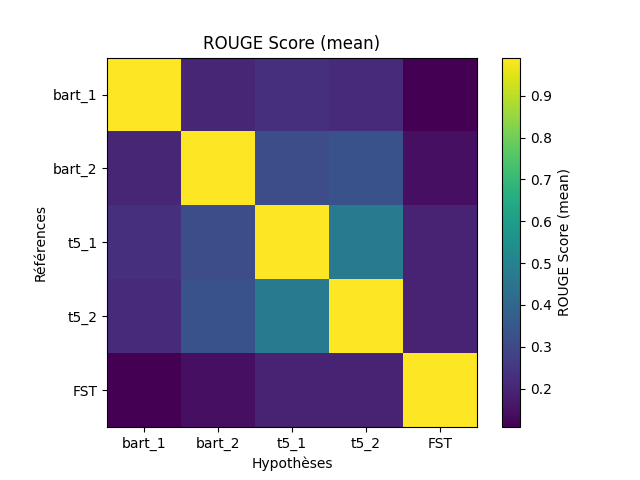
\includegraphics[width=0.35\textwidth]{images/rouge_score_mean_1000.png}
\caption{Moyenne de la métrique ROUGE sur un échantillon de 1000 phrases}
\label{fig}
\end{figure}

Les résultats présentés dans la figure \ref{fig} illustrent la comparaison effectuée à l'aide de la métrique ROUGE-1 sur un échantillon de 1000 phrases. On peut observer que les réponses générées par les modèles t5\_2 et t5\_1 sont très similaires (couleurs bleu), avec un score de similarité élevé (indice de 0.6). En revanche, les réponses générées par les modèles bart et FST sont nettement différentes, avec un score de similarité faible, ce qui indique l'absence de lien significatif entre leurs réponses respectives.

\subsection{Analyse des résultats avec ROUGE-N}

Dans cette section, nous avons calculé la moyenne des résultats de la métrique ROUGE-4 sur un ensemble de 1000 images commentées, ce qui permet de comparer les 4-grammes entre les différentes IA.

\begin{figure}[ht!]
\centering
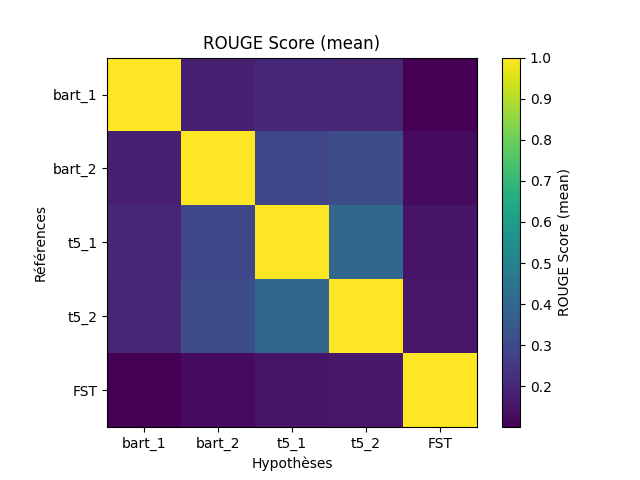
\includegraphics[width=0.35\textwidth]{images/rouge_score_mean_4.png}
\caption{Résultats de la métrique ROUGE-4 sur 1000 phrases}
\label{fig:rouge_score_mean_4}
\end{figure}

Les résultats présentés dans la figure \ref{fig:rouge_score_mean_4} confirment les tendances observées précédemment avec ROUGE-1. Les modèles t5\_1 et t5\_2 génèrent des phrases très similaires, ce qui peut s'expliquer par le fait qu'ils utilisent souvent les mêmes structures de génération.

\subsection{Analyse avec les métriques BLEU et METEOR}

En plus de la métrique ROUGE, nous avons également calculé les métriques BLEU et METEOR pour évaluer la similarité entre les phrases générées par les différentes IA.

La métrique BLEU (Bilingual Evaluation Understudy) mesure la qualité des reformulations, en se basant sur la précision des N-grammes tout en pénalisant la brièveté. Toutefois, cette métrique a tendance à pénaliser les phrases qui utilisent des mots moins courants. Dans notre étude, nous avons considéré une phrase de référence et nous avons comparé les phrases générées par les différentes IA pour une même image.\\

La métrique METEOR (Metric for Evaluation of Translation with Explicit ORdering) se base sur la moyenne harmonique et prend en compte la correspondance radicale et synonymique. Cette métrique est généralement plus précise que BLEU.\\

\begin{figure}[htbp!]
\centering
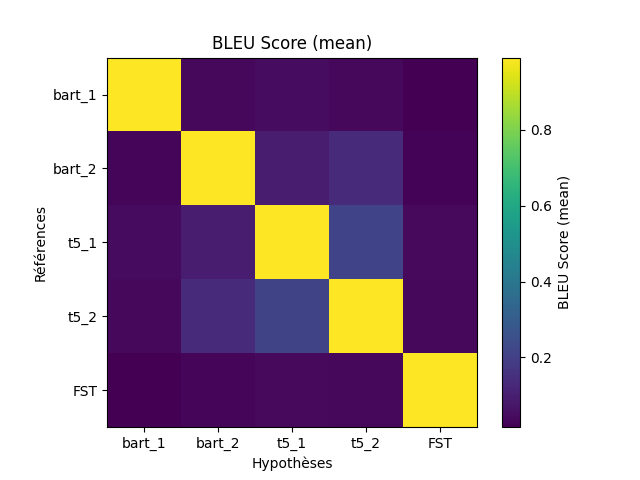
\includegraphics[width=0.35\textwidth]{images/bleu_score_mean_1000.png}
\caption{Moyenne des scores BLEU pour les phrases générées par les différentes IA}
\label{fig}
\end{figure}

\begin{figure}[htbp!]
\centering
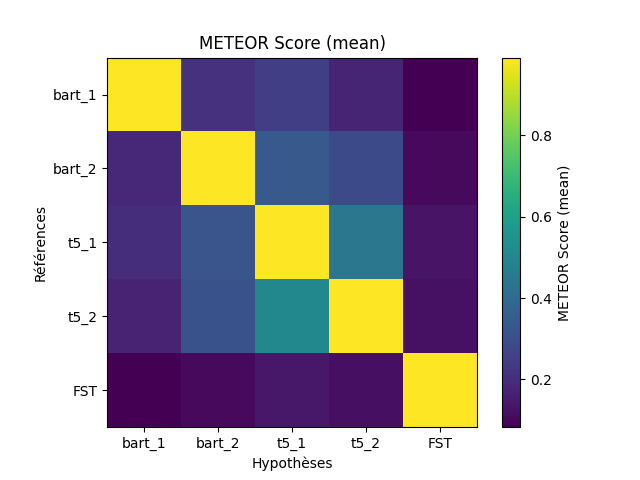
\includegraphics[width=0.35\textwidth]{images/meteor_score_mean_1000.png}
\caption{Moyenne des scores METEOR pour les phrases générées par les différentes IA}
\label{fig}
\end{figure}

Nous avons réalisé ces mesures sur un grand ensemble de phrases, ce qui nous a permis de moyenner les résultats et d'en tirer des conclusions générales. Les résultats obtenus avec les métriques BLEU et METEOR sont similaires à ceux obtenus avec ROUGE. On peut observer que les modèles t5\_1 et t5\_2 génèrent des phrases très proches pour une image donnée, tandis que les modèles bart\_1 et FST se démarquent avec des phrases moins similaires.

\subsection{Conclusion de l'analyse}

En résumé, notre analyse basée sur les métriques ROUGE, BLEU et METEOR a permis de mettre en évidence des similarités et des différences entre les phrases générées par les différentes IA pour une même image. Les modèles t5\_1 et t5\_2 génèrent des phrases très proches, tandis que les modèles bart\_1 et FST se distinguent par des phrases moins similaires. Ces résultats fournissent des indications précieuses sur le comportement des différentes IA et peuvent aider à sélectionner le modèle le plus adapté à une tâche spécifique.

% An example of a floating figure using the graphicx package.
% Note that \label must occur AFTER (or within) \caption.
% For figures, \caption should occur after the \includegraphics.
% Note that IEEEtran v1.7 and later has special internal code that
% is designed to preserve the operation of \label within \caption
% even when the captionsoff option is in effect. However, because
% of issues like this, it may be the safest practice to put all your
% \label just after \caption rather than within \caption{}.
%
% Reminder: the "draftcls" or "draftclsnofoot", not "draft", class
% option should be used if it is desired that the figures are to be
% displayed while in draft mode.

%\begin{figure}[!t]
%\centering
%\includegraphics[width=2.5in]{myfigure}
% where an .eps filename suffix will be assumed under latex, 
% and a .pdf suffix will be assumed for pdflatex; or what has been declared
% via \DeclareGraphicsExtensions.
%\caption{Simulation results for the network.}
%\label{fig_sim}
%\end{figure}

% Note that the IEEE typically puts floats only at the top, even when this
% results in a large percentage of a column being occupied by floats.


% An example of a double column floating figure using two subfigures.
% (The subfig.sty package must be loaded for this to work.)
% The subfigure \label commands are set within each subfloat command,
% and the \label for the overall figure must come after \caption.
% \hfil is used as a separator to get equal spacing.
% Watch out that the combined width of all the subfigures on a 
% line do not exceed the text width or a line break will occur.
%
%\begin{figure*}[!t]
%\centering
%\subfloat[Case I]{\includegraphics[width=2.5in]{box}%
%\label{fig_first_case}}
%\hfil
%\subfloat[Case II]{\includegraphics[width=2.5in]{box}%
%\label{fig_second_case}}
%\caption{Simulation results for the network.}
%\label{fig_sim}
%\end{figure*}
%
% Note that often IEEE papers with subfigures do not employ subfigure
% captions (using the optional argument to \subfloat[]), but instead will
% reference/describe all of them (a), (b), etc., within the main caption.
% Be aware that for subfig.sty to generate the (a), (b), etc., subfigure
% labels, the optional argument to \subfloat must be present. If a
% subcaption is not desired, just leave its contents blank,
% e.g., \subfloat[].


% An example of a floating table. Note that, for IEEE style tables, the
% \caption command should come BEFORE the table and, given that table
% captions serve much like titles, are usually capitalized except for words
% such as a, an, and, as, at, but, by, for, in, nor, of, on, or, the, to
% and up, which are usually not capitalized unless they are the first or
% last word of the caption. Table text will default to \footnotesize as
% the IEEE normally uses this smaller font for tables.
% The \label must come after \caption as always.
%
%\begin{table}[!t]
%% increase table row spacing, adjust to taste
%\renewcommand{\arraystretch}{1.3}
% if using array.sty, it might be a good idea to tweak the value of
% \extrarowheight as needed to properly center the text within the cells
%\caption{An Example of a Table}
%\label{table_example}
%\centering
%% Some packages, such as MDW tools, offer better commands for making tables
%% than the plain LaTeX2e tabular which is used here.
%\begin{tabular}{|c||c|}
%\hline
%One & Two\\
%\hline
%Three & Four\\
%\hline
%\end{tabular}
%\end{table}


% Note that the IEEE does not put floats in the very first column
% - or typically anywhere on the first page for that matter. Also,
% in-text middle ("here") positioning is typically not used, but it
% is allowed and encouraged for Computer Society conferences (but
% not Computer Society journals). Most IEEE journals/conferences use
% top floats exclusively. 
% Note that, LaTeX2e, unlike IEEE journals/conferences, places
% footnotes above bottom floats. This can be corrected via the
% \fnbelowfloat command of the stfloats package.




\section{Conclusion}
The conclusion goes here.




% conference papers do not normally have an appendix


% use section* for acknowledgment
\section*{Acknowledgment}


The authors would like to thank...





% trigger a \newpage just before the given reference
% number - used to balance the columns on the last page
% adjust value as needed - may need to be readjusted if
% the document is modified later
%\IEEEtriggeratref{8}
% The "triggered" command can be changed if desired:
%\IEEEtriggercmd{\enlargethispage{-5in}}

% references section

% can use a bibliography generated by BibTeX as a .bbl file
% BibTeX documentation can be easily obtained at:
% http://mirror.ctan.org/biblio/bibtex/contrib/doc/
% The IEEEtran BibTeX style support page is at:
% http://www.michaelshell.org/tex/ieeetran/bibtex/
%\bibliographystyle{IEEEtran}
% argument is your BibTeX string definitions and bibliography database(s)
%\bibliography{IEEEabrv,../bib/paper}
%
% <OR> manually copy in the resultant .bbl file
% set second argument of \begin to the number of references
% (used to reserve space for the reference number labels box)
\begin{thebibliography}{1}

\bibitem{IEEEhowto:kopka}
H.~Kopka and P.~W. Daly, \emph{A Guide to \LaTeX}, 3rd~ed.\hskip 1em plus
  0.5em minus 0.4em\relax Harlow, England: Addison-Wesley, 1999.

\end{thebibliography}




% that's all folks
\end{document}
